\question[6]如图,水平放置的圆柱形光滑玻璃棒左边绕有一线圈,右边套有一金属圆环。圆环初始时静止。将图中开关S由断开状态拨至连接状态,电路接通的瞬间,可观察到\key{B}\begin{center}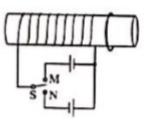
\includegraphics[width=4cm]{img/image1.png}\end{center}
\fourchoices{拨至M端或N端,圆环都向左运动}{拨至M端或N端,圆环都向右运动}{拨至M端时圆环向左运动,拨至N端时向右运动}{拨至M端时圆环向右运动,拨至N端时向左运动}
\begin{solution}{4cm}

\end{solution}



\question[6]甲、乙两个物块在光滑水平桌面上沿同一直线运动,甲追上乙,并与乙发生碰撞,碰撞前后甲、乙的速度随时间的变化如图中实线所示。已知甲的质量为$1kg$,则碰撞过程两物块损失的机械能为\key{A}\begin{center}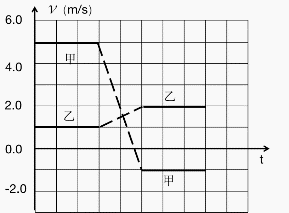
\includegraphics[]{img/image2.png}\end{center}
\fourchoices{3J}{4J}{5J}{6J}
\begin{solution}{4cm}

\end{solution}



\question[6]"嫦娥四号"探测器于$2019$年1月在月球背面成功着陆,着陆前曾绕月球飞行,某段时间可认为绕月做匀速圆周运动,圆周半径为月球半径的K倍。已知地球半径R是月球半径的Р倍,地球质量是月球质量的Q倍,地球表面重力加速度大小为g。则"嫦娥四号"绕月球做圆周运动的速率为\key{D}
\fourchoices{$\sqrt{\frac{RKg}{QP}}$}{$\sqrt{\frac{RPKg}{Q}}$}{$\sqrt{\frac{RQg}{KP}}$}{$\sqrt{\frac{RPg}{QK}}$}
\begin{solution}{4cm}

\end{solution}



\question[6]如图,悬挂甲物体的细线拴牢在一不可伸长的轻质细绳上O点处;绳的一端固定在墙上,另一端通过光滑定滑轮与物体乙相连。甲、乙两物体质量相等。系统平衡时,O点两侧绳与竖直方向的夹角分别为α和β。若$α=70^∘$,则β等于\key{B}\begin{center}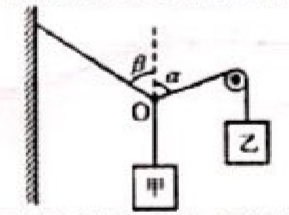
\includegraphics[width=4cm]{img/image3.png}\end{center}
\fourchoices{$45°$}{$55°$}{$60°$}{$70°$}
\begin{solution}{4cm}

\end{solution}



\question[6]真空中有一匀强磁场,磁场边界为两个半径分别为a和3a的同轴圆柱面,磁场的方向与圆柱轴线平行,其横截面如图所示。一速率为ν的电子从圆心沿半径方向进入磁场。已知电子质量为m,电荷量为e,忽略重力。为使该电子的运动被限制在图中实线圆围成的区域内,磁场的磁感应强度最小为\key{C}\begin{center}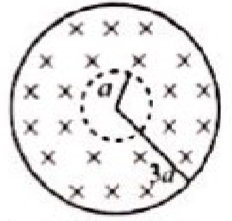
\includegraphics[width=4cm]{img/image4.png}\end{center}
\fourchoices{$\frac{3mv}{2ae}$}{$\frac{mv}{ae}$}{$\frac{3mv}{4ae}$}{$\frac{3mv}{5ae}$}
\begin{solution}{4cm}

\end{solution}



\question[6]$1934$年,约里奥—居里夫妇用α粒子轰击铝箔,首次产生了人工放射性同位素X,反应方程为:$_{2}^{4}He+_{13}^{27}Al\rightarrow X+_0^1n$。X会衰变成原子核Y,衰变方程为$X→Y+_1^0e$,则\key{AC}
\fourchoices{X的质量数与Y的质量数相等}{X的电荷数比Y的电荷数少1}{X的电荷数比的电荷数多2}{X的质量数与的质量数相等}
\begin{solution}{4cm}

\end{solution}


\newpage
\question[6]在图(a)所示的交流电路中,电源电压的有效值为$220V$,理想变压器原、副线圈的匝数比为10:1,$R_1$、$R_2$、$R_3$均为固定电阻,$R_2=10$,$R_3=20$,各电表均为理想电表。已知电阻$R_2$中电流$i_2$随时间t变化的正弦曲线如图(b)所示。下列说法正确的是\key{AD}\begin{center}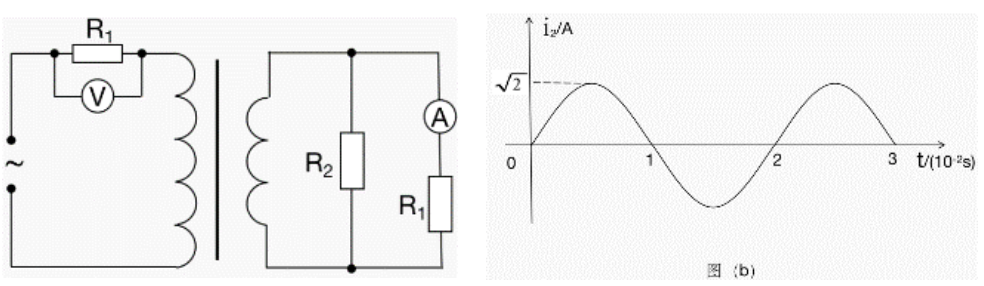
\includegraphics[width=14cm]{img/image5.png}\end{center}
\fourchoices{所用交流电的频率为$50Hz$}{电压表的示数为$100$}{电流表的示数为$1.0A$}{变压器传输的电功率为$15.0W$}
\begin{solution}{4cm}

\end{solution}



\question[6]如图,$\angle M$是锐角三角形$PMN$最大的内角,电荷量为q($q>0$)的点电荷固定在Р点。下列说法正确的是\key{BC}\begin{center}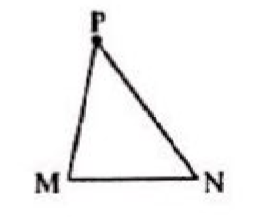
\includegraphics[width=4cm]{img/image6.png}\end{center}
\fourchoices{沿M边,从M点到M点,电场强度的大小逐渐增大}{沿M边,从M到N点,电势先增大后减小}{正电荷在M值点的电势能比其在M点的电势能大}{将正电荷从M点移动到M点,电场力所做的总功为负}
\begin{solution}{4cm}

\end{solution}


\newpage
